\begin{figure}[htbp]
  \centering
  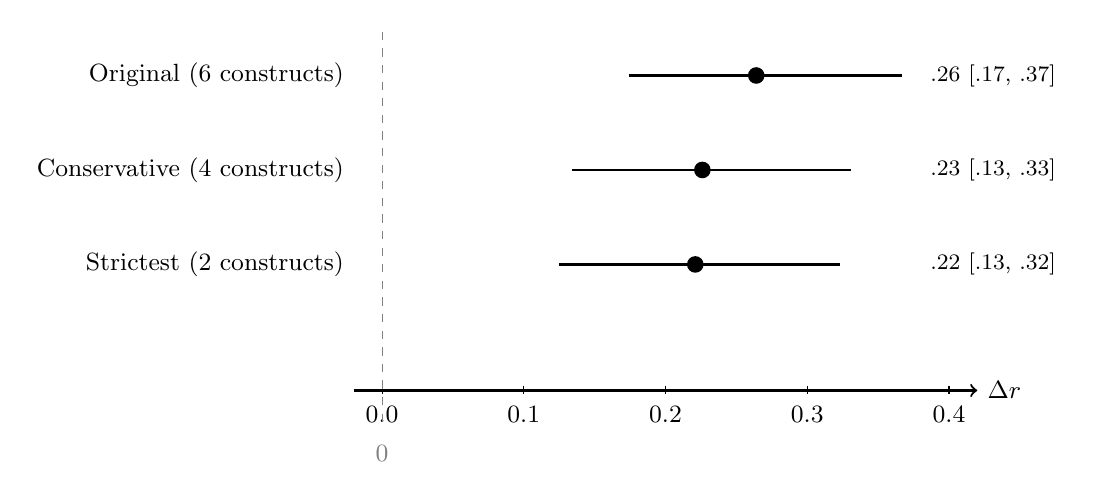
\begin{tikzpicture}[x=18cm,y=1cm,font=\small]
    % --- Axis ---
    \draw[->,thick] (-0.02, 0) -- (0.42, 0) node[right] {$\Delta r$};
    \foreach \x in {0.0, 0.1, 0.2, 0.3, 0.4} {
      \draw (\x, 0.05) -- (\x, -0.05);
      \node[below=1pt] at (\x, -0.05) {\(\x\)};
    }
    \draw[dashed,gray] (0, -0.4) -- (0, 4.6);
    \node[below=15pt,gray] at (0, -0.05) {0};

    % --- Reference line at 0 ---

    % --- Row 1: Original (6) ---
    \node[anchor=east] at (-0.02, 4) {Original (6 constructs)};
    \draw[thick] (0.174, 4) -- (0.367, 4);
    \fill (0.264, 4) circle (3pt);
    \node[anchor=west,font=\footnotesize] at (0.38, 4) {$.26$ [.17, .37]};

    % --- Row 2: Conservative (4) ---
    \node[anchor=east] at (-0.02, 2.8) {Conservative (4 constructs)};
    \draw[thick] (0.134, 2.8) -- (0.331, 2.8);
    \fill (0.226, 2.8) circle (3pt);
    \node[anchor=west,font=\footnotesize] at (0.38, 2.8) {$.23$ [.13, .33]};

    % --- Row 3: Strictest (2) ---
    \node[anchor=east] at (-0.02, 1.6) {Strictest (2 constructs)};
    \draw[thick] (0.125, 1.6) -- (0.323, 1.6);
    \fill (0.221, 1.6) circle (3pt);
    \node[anchor=west,font=\footnotesize] at (0.38, 1.6) {$.22$ [.13, .32]};

  \end{tikzpicture}
  \caption{Tautology sensitivity analysis for the hostile aggression advantage. Each row shows the bootstrap-estimated difference between $r_\textit{hostile~aggression}$ and $r_\textit{crime~concerns}$ in predicting the punitiveness aggregate, with 95\% bias-corrected and accelerated (BCa) confidence intervals (10{,}000 iterations). The three rows correspond to progressively stricter operationalizations of the hostile aggression cluster: \textit{Original} retains all six constructs (exclusion, degradation, suffering, prison violence tolerance, harsh conditions, revenge); \textit{Conservative} drops the two most punishment-tautological (suffering and harsh conditions); \textit{Strictest} retains only social exclusion and revenge. All three intervals exclude zero, indicating that the hostile aggression advantage is not an artifact of construct overlap with the punitiveness measures. $N = 496$.}
  \label{fig:bootstrap}
\end{figure}
